\documentclass[12pt,a4paper]{scrartcl}

\usepackage{hyperref}
\usepackage{url}
\usepackage{graphicx}
\usepackage{xcolor}
\usepackage{textcomp}
\usepackage{subfig}

\newcommand{\obtain}[0]{\textcolor{orange}{\textbf{obtain}}}
\newcommand{\avail}[0]{\textcolor{green}{\textbf{available}}}
\newcommand{\build}[0]{\textcolor{red}{\textbf{build}}}
\newcommand{\code}[0]{\textcolor{blue}{\textbf{code}}}


\parskip 0.3 cm
\parindent 0 cm

\title{QTB PBR Hack`a'thing}
\subtitle{Soldering for and by beginners.}
\date{March 2--4, 2016}

\begin{document}
\maketitle
%\scriptsize
\tableofcontents
%\normalsize
\newpage

\section{PBR Hack`a'thing Projects}
\label{proj}

\begin{figure}[ht]
  \begin{minipage}{.49\textwidth}
    \subfloat[Dougie's Reactor]{
      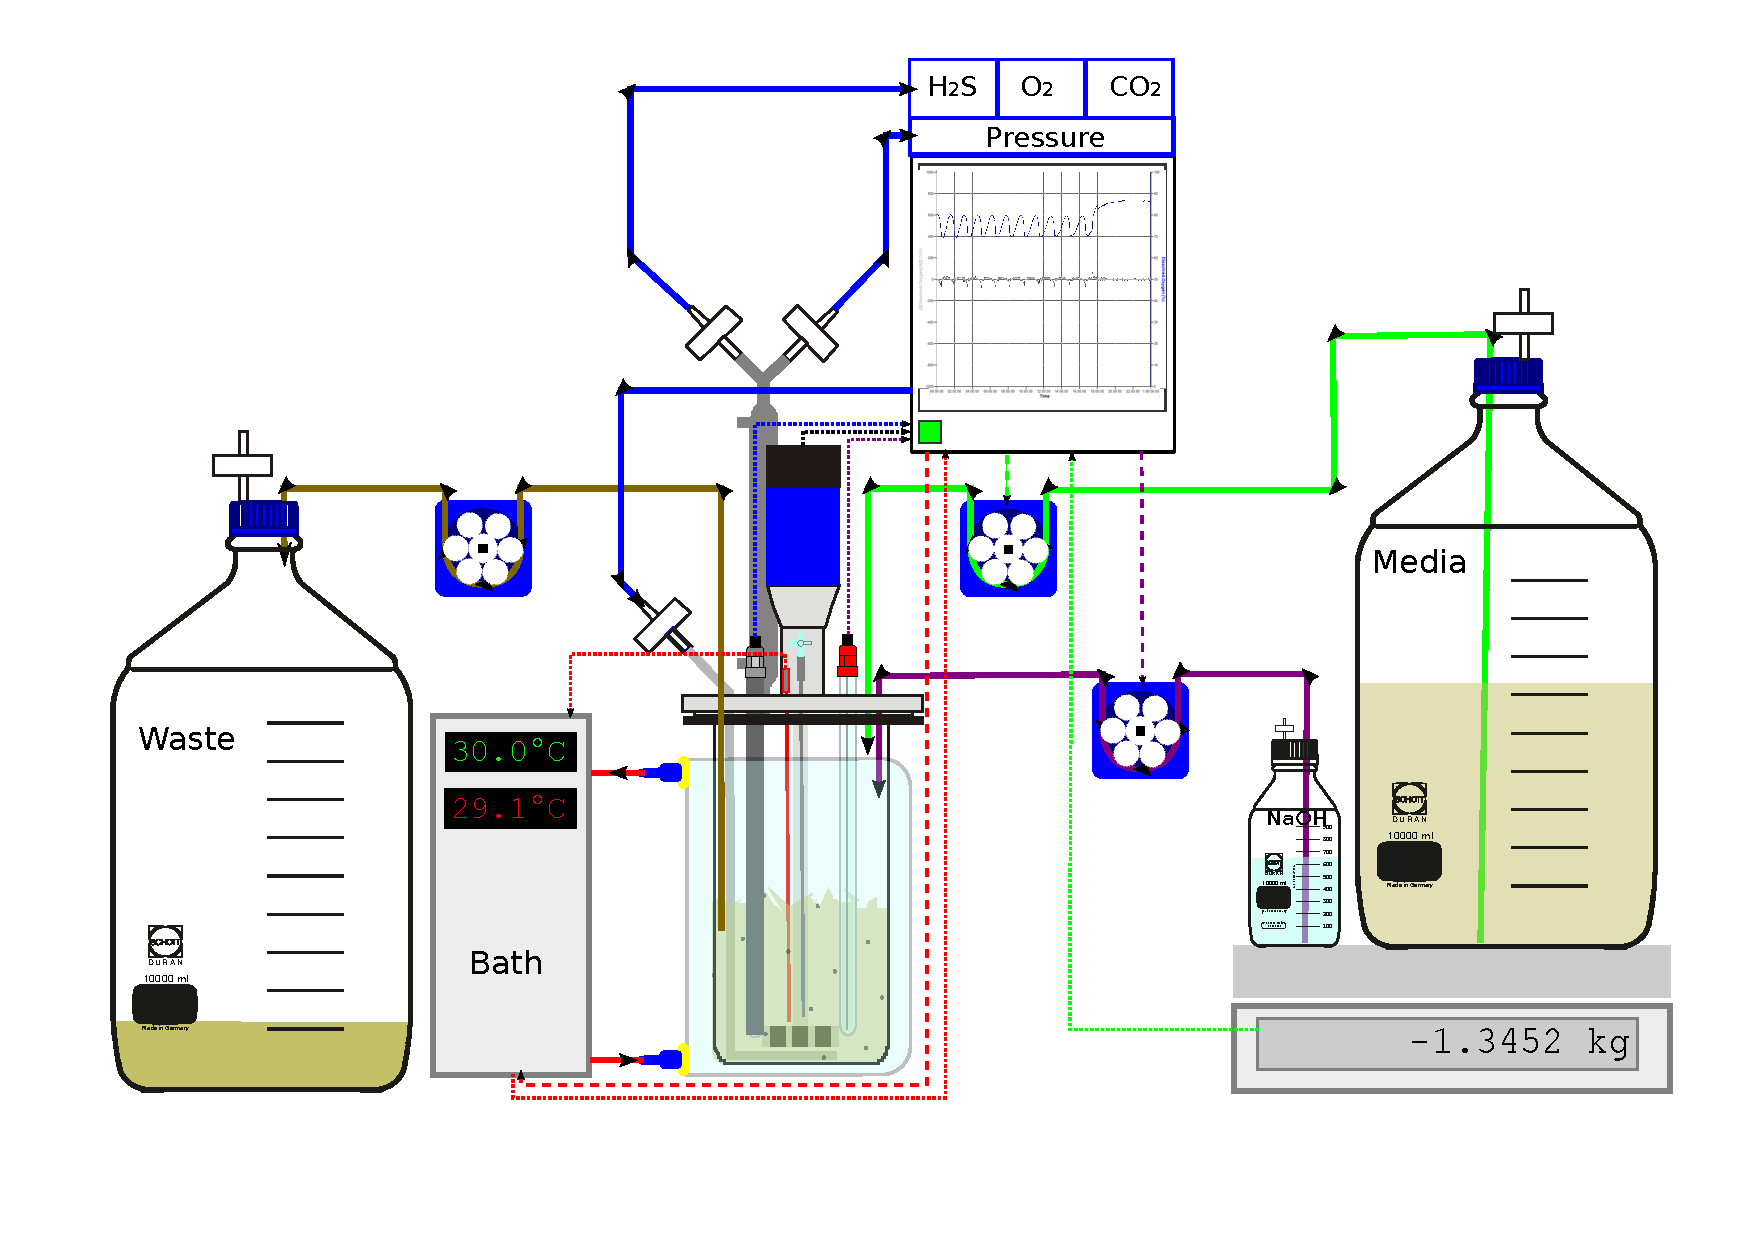
\includegraphics[width=\textwidth]{figures/fermentor_detailed.pdf}\\ 
    }
  \end{minipage}
  \begin{minipage}{.49\textwidth}
    \centering Monod: $\mu = \mu_{max} \frac{S}{S+K_S}$\\
    \subfloat[Snoep \textit{et al.} 2009]{
      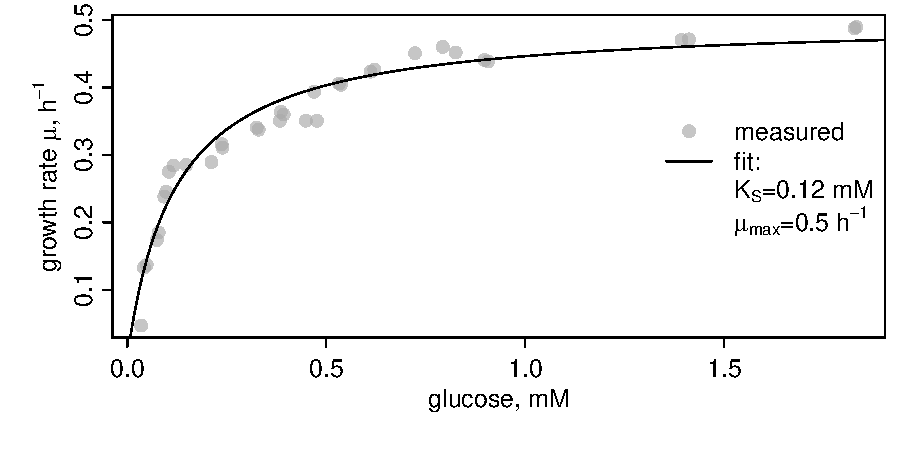
\includegraphics[width=\textwidth]{figures/snoep09_fig2.pdf}
    }
  \end{minipage}
\caption[]{Bioreactors}
\end{figure}


\subsection{Gas Flux: Gasometer}
\label{gas}
\paragraph{Project:} 
Extend existing setup, co2meter's
\href{http://www.co2meter.com/collections/co2-sensors/oxygen-sensors}{O2}
and
\href{http://www.co2meter.com/collections/co2-sensors/products/cozir-5-100-co2-sensor}{CO2}
sensors with Sainsmart's
\href{http://www.sainsmart.com/featured-products/sainsmart-mega2560-board-3-5-tft-lcd-module-display-shield-kit-for-atmel-atmega-avr-16au-atmega8u2.html}{Arduino
  Mega+Touch screen}; see directory \texttt{offgas/arduino} in
\url{https://git.hhu.de/machne/PSIControl} for Arduino code

\begin{enumerate}
\item \code{} sensor calibration routines via touch-screen (use PSI
  gas mixing system)
\item \build{} water trap, tubing path from reactor, and casing for
  sensors and Arduino; \build{} improved gassing system (glas
  blowers!) to allow lower flow
\item \build{} \& \code{} interface to \href{http://www.aalborg.com/index.php/main_page/product_overview/id_product_overview/63}{Aalborg XFM digital mass flow
  meter}: connect the Aalborg's RS 485 interface to Arduino hardware
  serial Tx3,Rx3
\item \build{} \& \code{} valve control to measure several reactors;
  connect via Arduino software serial connections; perhaps attach to
  PSI Multicultivator
\end{enumerate}

\paragraph{Materials:}

\begin{itemize}
\item Existing setup: \avail{}
\item Aalborg XFM, with RS 485 interface: \avail{}
\item Valve system for gas tubing, controllable \textit{via} serial
  interface: \obtain{}
\end{itemize}

\subsection{Liquid Flux: Continuous Culture \& Turbidostat} 
\label{cult}

\paragraph{Project:} build a module consisting of media and waste bottles, a reactor vessel, peristaltic pump(s), and a balance; pump and balance are controlled  \textit{via} serial interfaces from  an Arduino+Touchscreen and/or
Raspberry Pi. The flow rate is controlled \textit{via} pump and
recorded \textit{via} the balance, dilution rate (depends on culture
volume) is recorded or can be set.

\begin{enumerate}
\item \build{} a simple reactor vessel (Schott bottles) with liquid
  media flow, from media bottles through reactor vessel and out to
  waste bottle; connect \textit{via} tubing and pumps, record
  \textit{via} balance
\item Add gassing system of project \ref{gas}
\item Combine with \ref{spec} to make turbidostatic control
\end{enumerate}


\paragraph{Materials:}
\begin{itemize}
\item Media bottlesm, screw caps with inlet/outlet openings,
  and tubing: \avail{} in the lab, but check!
\item Balance (e.g. Mettler Toledo
\href{http://de.mt.com/de/de/home/products/Industrial_Weighing_Solutions/bench-scales/weighing-platforms/high-resolution/PBK785.html}{PBK785-3XS/f}): \obtain{}
\item Peristaltic pumps: ordered?
\item Arduino: \obtain{}
\end{itemize}

\subsection{Light Flux: Spectrometer} 
\label{spec}
\paragraph{Project:} 
Simple spectrometric measuring tool based on
\href{http://www.avantes.com/products/spectrometers/compactline/item/723-avaspec-mini}{AvaSpec-Mini2048l-U25}

\begin{enumerate}
\item Basic: Connect to Rasperry Pi, using drivers provides by
  Avantes; \code{} simple interface with display and/or recording
  functions
\item Advanced: use LED for absorbance, reflectance, or fluorescence
  measurements; \build{} light paths and perhaps a reactor probe for
  online recording
\end{enumerate}

\paragraph{Materials:}
\begin{itemize}
\item AVASPEC-MINI2048L-V25, Minispectrometer: \avail{}
\item Fiber optic cables, VIS/NIR: 1 m, 200 \textmu{}m VIS/NIR and 1m,
  600 \textmu{}m: \avail{}
\item Raspberry Pi Version 1: \obtain{}
\item LED system: use PSI LEDs or \obtain{}
\item Reactor probe: \build{} together with fine mechanics or glas
  blowers
\end{itemize}


\subsection{Heat Flux: Water Bath Thermostat}
\label{heat}

\paragraph{Project:} build a water bath for growth vessels, control
T, read-out energy required for maintaining constant T and estimate
the amount of heat withdrawn or administered

\begin{enumerate}
\item
\end{enumerate}

\paragraph{Materials:}
\begin{itemize}
\item Jacketed reactor vessel: \build{} or \obtain{}
\item Julabo water bath,
e.g. \href{http://www.laborhandel24.de/9162625-de?utm_source=google_shopping&gclid=Cj0KEQiA496zBRDoi5OY3p2xmaUBEiQArLNnK6uWkryhjvkNdmRLgcg2W_HIO9W1aKaKCO9gmvlkt_MaAmhe8P8HAQ}{F25-ME}
\item Arduino and/or Raspberry Pi
\end{itemize}

\subsection{Single Cell Biology: Microfluidics Device} 
\label{micro}

\paragraph{Project:} Basic microfluidics and live-cell imaging device;
scratch growth chambers and liquid flow channgels into microscope slide;
attach 2--3 pumps; and control \textit{via} arduino/screen

\paragraph{Materials:}
\begin{itemize}
\item Ilka's lab microscope: \avail{}
\item Microscopy slides: \avail{}
\item 2--3 peristaltic pumps for microfluidics: \obtain{}
\item Sainsmart's Arduino Mega + Touchscreen: \obtain{}
\end{itemize}


\newpage

\section{Program}

\subsection{Day 1 $<$12:00 : Building Bioreactors}

Talks, 30-60 min:

\subsubsection{Rob's DIY Reactor - The Beginnings}

The Captor - Arduino-controlled mini PBR

\subsubsection{Dougie's DIY Reactor - 20 yrs Later}
\subsubsection{Avantes - Spectrometry}

Spectrometry applications, incl. NIR for metabolite measurements and OD

Software interface to Avantes spectrometers

\subsubsection{CellDeg - Optimizing Photosynthetic Growth}

Introduction to CellDeg's 2.5 k Euro algal growth setup (overnight 30 g/L
cyano biomass)

\subsection{Day 1 $>$13:00 : Hack`a'thing I}

Introduction to the gasometer: connecting sensors with Arduino,
making an autonomous measurement device via Sainsmart's Touch Screen

Introduction to Rob's reactor: complete setup for photosynthetic growth

Self-organizing into teams: lab hardware (tubing etc.), control hardware
(soldering etc.), software

\subsection{Day 2 $<$12:00 : Photobioreactors in Research}

Talks, 30-60 min:

Nir Keren, Hellingwerf, Jan Cerveny, Dougie Murray,
something microfluidics?

\subsection{Day 2 $>$13:00 : Hack`a'thing II}

Perhaps in teams, either by projects (\ref{gas}--\ref{micro}) or in
software vs. hardware (soldering/tubing) vs. biolab (cell cultures),
or -- most likely -- in dynamic self-organisation, working parallel on
all projects.

\subsubsection{Hardware I} 
soldering, tubing

\subsubsection{Software I} 
probe/sensor/pump $\Leftrightarrow$ arduino/raspi interfaces

\subsection{Day 3 $<$12:00 : Hack`a'thing III}

\subsubsection{Hardware II} 
Integrate projects \ref{gas},\ref{spec}\&\ref{cult} into a simple DIY
reactor and/or with PSI FMT150 or Multicultivator

Integrate project \ref{micro} with the simple microscope in Ilka's lab,
or a more advanced system (CAi?)

Visit HHU's fine mechanics and glas blower work-shops, place orders 
for stuff missing for above goals


\subsection{Day 3 $>$13:00 : Consolidating}

\subsubsection{Software II}
arduino/raspi $\Leftrightarrow$  master/server interface

Standard data formats and interfaces

Brain storming: relation of data and models

Beer: relation of data and models and beer


\end{document}
